\chapter{Bacterial chromatin, FtsZ, and other projects}\label{other_projects}

My PhD project was originally focused on unraveling the structure and function of the nucleoid-associated protein HU, and its role in chromatin compaction and nucleoid dynamics in \textit{D. radiodurans}.
The structural study of FtsZ --- both in STA and SPA --- emerged from our exploration of the nucleoid and cell dividion processes of \textit{D. radiodurans} in cryo-ET as part of the septation paper (\fullref{drad})
Along the way, I contributed to a few other projects and developed several tools.
This chapter presents these projects and the tools and scripts worthy of mention in this manuscript.

\localtableofcontents

\section{Bacterial chromatin and HU}\label{hu}

Initially the main project of my PhD, the study of bacterial chromatin compaction by cryo-EM and cryo-ET is an ongoing project in the MICA group, which builds upon previous fluorescence imaging on \textit{D. radiodurans} done by the GenOM team nucleoids and more recent cryo-EM and cryo-ET data collected and prepared by the MICA team.
The main protein of interest is HU, a nucleoid-associated protein (NAP) present in most bacteria (including \textit{E. coli} and \textit{D. radiodurans}) which is known to be a key player in chromatin compaction and nucleoid morphology throughout the cell cycle.
The structure of dimeric HU has been solved from various bacterial species in either its apo- or DNA-bound forms (\autoref{fig:hu}).
HU is thought to have a histone-like function --- with molecular dynamics simulations supporting the evidence to this binding mode~\cite{hognonMolecularBasesDNA2019} --- but it was also observed forming stacks of dimers that lay parallel to the DNA duplex, suggesting the possibility of multiple modes of interaction between HU dimers and the DNA~\cite{hammelHUMultimerizationShift2016}.
Such drastically different modes may explain the heterogeneous highly dynamic nature of the \textit{D. radiodurans} nucleoids despite the relatively low number of players involved --- mostly just HU and a DNA-gyrase~\cite{TODO}.

\begin{figure}[ht]
    \centering
    \begin{subfigure}[B]{.48\textwidth}
        \centering
        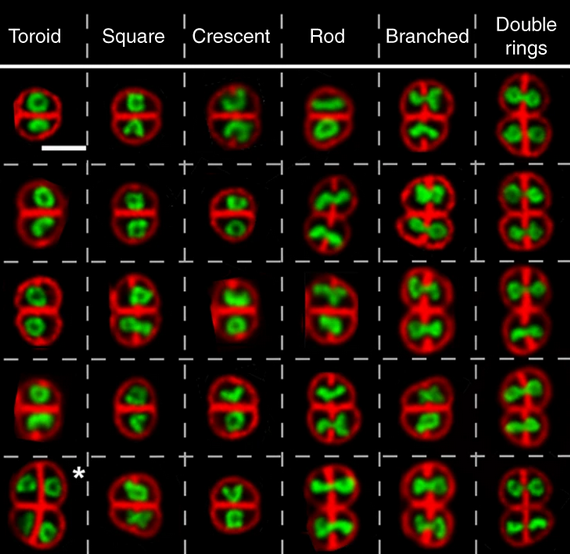
\includegraphics[width=\textwidth]{other/dr_nucleoids.png}
        \caption{\textit{D. radiodurans} heterogeneous and dynamic nucleoid morphology shows variations throughout the cell cycle. Figure taken from \citet{flochCellMorphologyNucleoid2019}.}
        \label{fig:hu_nucleoids}
    \end{subfigure}%
    \hfill
    \begin{subfigure}[B]{.5\textwidth}
        \centering
        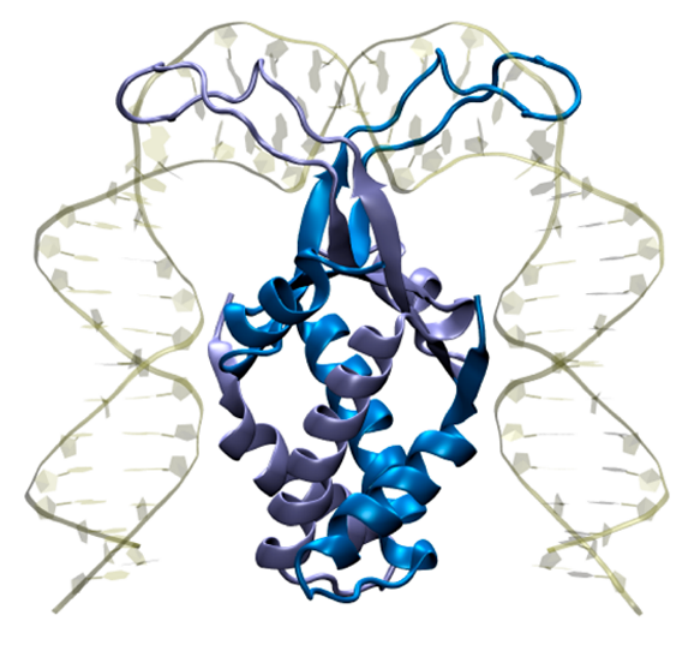
\includegraphics[width=\textwidth]{other/hu_struct.png}
        \caption{\textit{Borrelia burgdorferi} HU structure determined by X-ray crystallography. Its DNA-kinking histone-like behavior was replicated by molecular dynamics simulations. Figure taken from \citet{hognonMolecularBasesDNA2019}.}
        \label{fig:hu_structure}
    \end{subfigure}%
    \titledcaption[\textit{D. radiodurans} nucleoids and HU structure]{\textbf{(a)} Nucleoid compaction and morphology in \textit{D. radiodurans} is complex and dynamic, with HU being one of the major drivers of chromatin compaction. \textbf{(b)} HU is thought to have a histone-like behaviour, bending the DNA to form a tight kink.}
    \label{fig:hu}
\end{figure}

To begin investigating DrHU in complex with the DNA, we collected single particle cryo-EM data of an \textit{in vitro} preparation of plasmid DNA and HU, in order to observe the interaction in a free aqueous environment.
The bacterial genomic DNA is large, circular and supercoiled; where previous structural studies used short DNA segments, we opted for a circular dsDNA plasmid as it would be a more appropriate stand-in that would allows us to evaluate how circularity, supercoiling and DNA topology affect HU binding and assembly on DNA.
HU and plasmid DNA were mixed at different ratios, and within a small range of relative concentration (\sim100 HU/plasmid) intriguing spirals (\autoref{fig:hu_spirals}) were formed by the DNA.
Notably, these spirals were never observed in the absence of HU, and were also not observed when using older batches of the plasmid. % TODO: what does this mean? What older batch?

\begin{figure}[ht]
    \centering
    \includegraphics[width=\textwidth]{other/hu_spirals_no_spirals.png}
    \titledcaption[HU-induced DNA spirals]{Spiral formations of DNA are formed in presence of HU only at specific concentration ranges.}
    \label{fig:hu_spirals}
\end{figure}

The very small molecular weight of HU (\sim25 kDa in its dimeric form) meant that picking and processing these particles (even in the expected dimeric or tetrameric forms) would be practically impossible in cryo-EM (see \autoref{fig:et_smallest_particle} for the theoretical limits).
However, due to the relatively high concentration of HU --- \sim100 HU/plasmid corresponds to approximately 1 HU for every 26bp --- the DNA should be densely decorated by HU, unless the protein distribution on the grid is not uniform or big aggregates are forming.
It should therefore be possible to work around the particle size limitation by using the supporting geometry of the DNA filament to do the picking and guide refinement.

With this in mind, we devised two picking strategies: a DNA-aligned one (\autoref{fig:hu_picks_ondna}), from which we might be able to isolate picks where HU is decorating the DNA on the side, and one positioned between two DNA strands (\autoref{fig:hu_picks_betweendna}), where we might be able to see tetramer of HU, hypothesized to form a bridge between DNA filaments based on previous biochemical studies by the GenOM team.

, using two different templates: , and .

\begin{figure}[ht]
    \centering
    \begin{subfigure}[B]{.49\textwidth}
        \centering
        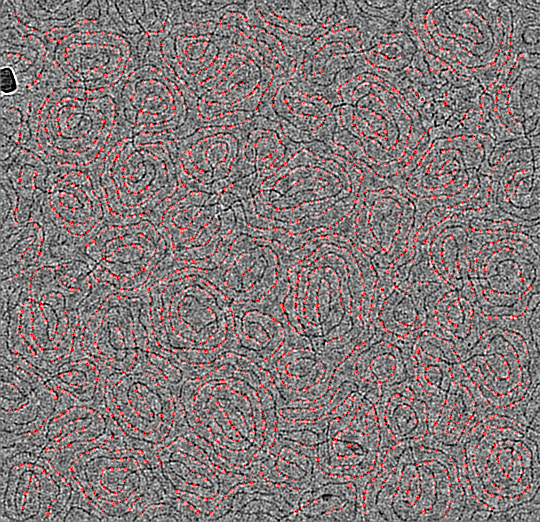
\includegraphics[width=\textwidth]{other/hu_picks_ondna.png}
        \caption{Particle picks aligned on the DNA.}
        \label{fig:hu_picks_ondna}
    \end{subfigure}%
    \hfill
    \begin{subfigure}[B]{.49\textwidth}
        \centering
        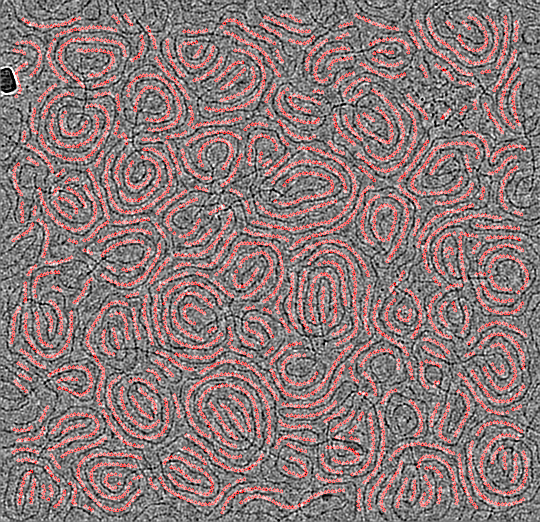
\includegraphics[width=\textwidth]{other/hu_picks_betweendna.png}
        \caption{Particle picks between DNA filaments.}
        \label{fig:hu_picks_betweendna}
    \end{subfigure}%
    \titledcaption[Filament picking strategies for HU]{Filament picking is controlled via several parameters, among which an optional template. We generated two different templates (by doing some manual picking and simple classification): one that is aligned with the DNA filament, and one centered between two DNA filaments. Particles picked using the CryoSPARC~\cite{punjaniCryoSPARCAlgorithmsRapid2017} filament picker.}
    \label{gih:hu_picks}
\end{figure}

With these picks and a few rounds of 2D classification and cleaning, we were able to obtain 2D in which DNA features were clearly visible; unfortunately, no decoration on the DNA was visible (\autoref{fig:hu_classes}).

\begin{figure}[ht]
    \centering
    \begin{subfigure}[B]{.49\textwidth}
        \centering
        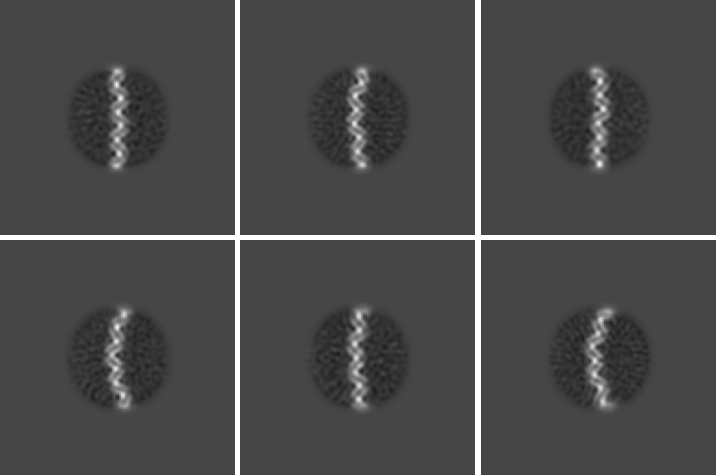
\includegraphics[width=\textwidth]{other/hu_classes_ondna.png}
        \caption{2D classes aligned on the DNA.}
        \label{fig:hu_classes_ondna}
    \end{subfigure}%
    \hfill
    \begin{subfigure}[B]{.49\textwidth}
        \centering
        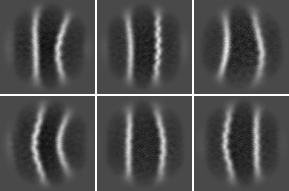
\includegraphics[width=\textwidth]{other/hu_classes_betweendna.png}
        \caption{2D classes between DNA filaments.}
        \label{fig:hu_classes_betweendna}
    \end{subfigure}%
    \titledcaption[2D classes from filament picking]{Particle picks aligned on the DNA show high resolution detail in the 2D classes, where the DNA double strand is clearly visible. Picks centered between two filaments did not reach as high resolutions, likely due to how impactful the relative spacing and curvature of the two DNA filaments is on driving the classification procedure.}
    \label{fig:hu_classes}
\end{figure}

We attempted also to pick particle manually or using topaz, focusing on each occurrence of a small "blob" of HU-compatible dimensions appearing next to the DNA (\autoref{fig:hu_topaz}).

\begin{figure}[]
    \centering
    \begin{subfigure}[B]{.5\textwidth}
        \centering
        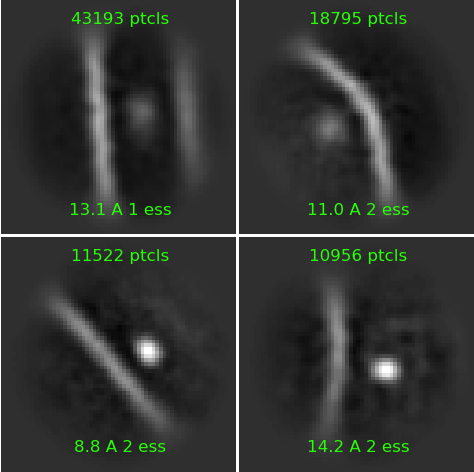
\includegraphics[width=\textwidth]{other/hu_topaz_classes.png}
        \caption{2D classes from Topaz picking.}
        \label{fig:hu_topaz_classes}
    \end{subfigure}%
    \hfill
    \begin{subfigure}[B]{.5\textwidth}
        \centering
        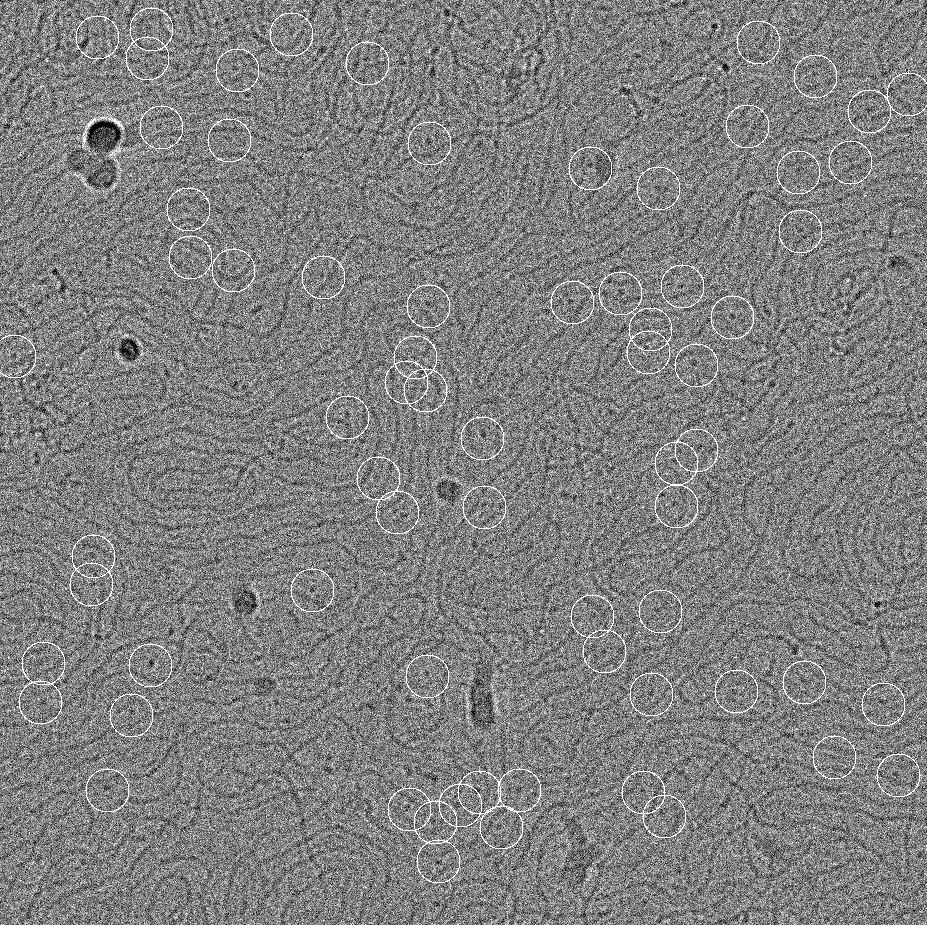
\includegraphics[width=\textwidth]{other/hu_topaz_picks.png}
        \caption{Particle picks from Topaz.}
        \label{fig:hu_topaz_picks}
    \end{subfigure}%
    \titledcaption[2D classification from Topaz picking]{Representative classification results (left) from Topaz picks (right) centered on "blobs" next to the DNA.}
    \label{fig:hu_topaz}
\end{figure}

In all these cases, when doing 3D reconstruction, we attempted to tight masking around the filament or next to it, or to restrict the refinement shifts to allow the DNA to help with initial alignement without hindering the pose refinement.
Unfortunately, in none of these cases we were able to successfully identify HU in our dataset, likely due to the small size of HU, but also the heterogeneous and dynamic nature of the HU-DNA complex.


\section{FtsZ function and structure}\label{ftsz}

To better understand the role of FtsZ in the septation of \textit{D. radiodurans}, we investigated its structure and superstructure using both single particle cryo-EM and \textit{in situ} cryo-ET.
This work is ongoing and not yet consolidated into a manuscript for publication.
Sample preparation and screening was performed by my supervisors Irina Gutsche and Joanna Timmins, while data collections were done partly by Irina, and partly commissioned to external facilities.
Data processing on the single particle and tomography data, and software tool development were performed by me.

\subsection{State of the art}

FtsZ is an extremely well conserved prokaryotic tubulin homologue, known to form ring-like structures (the Z-ring) at the septation site in most bacteria.
It polymerizes in a GTP-dependent fashion to form filaments and bundles, anchoring to the membrane via its partner FtsA, and interacting with several other partners in the cytokinesis and peptidoglycan (PG) synthesis machinery~\cite{barrowsFtsZDynamicsBacterial2021,mcquillenInsightsStructureFunction2020}.

Based on crystal structures, filaments have been shown to form through head-to-tail stacking of monomers CITE.
However, there is no structural information regarding the flexible C-terminal region, which is responsible for regulating its activity and interaction with its cellular partners, including FtsA.
It's also unclear how multiple filaments may assemble to form bundles at the structural level and even less so in vivo.
Thus --- while its key role in cell division is undisputed --- the exact mechanism and function of FtsZ are still unclear.
There is currently no consensus model that fully explains the function and mode of action of FtsZ in the division process in bacteria, as the current evidence is inconclusive, sometimes presenting significant variations between species --- likely ascribable to different shapes or membrane compositions between bacteria~\cite{barrowsFtsZDynamicsBacterial2021,mcquillenInsightsStructureFunction2020}.

\begin{figure}[ht]
    \centering
    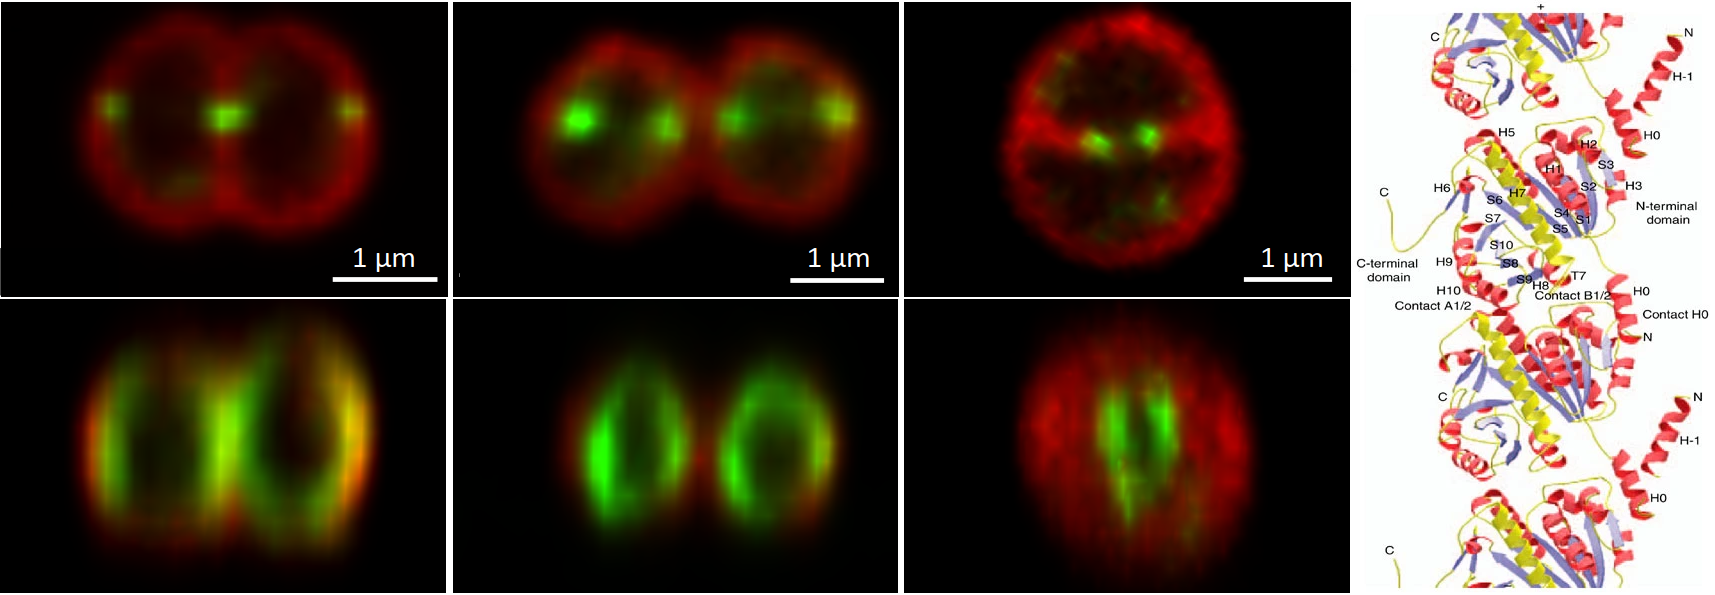
\includegraphics[width=\textwidth]{other/ftsz_ring.png}
    \titledcaption[FtsZ forms a ring \textit{in vivo} and filaments \textit{in vitro}]{During cell division, FtsZ is known to localize on a ring (termed Z-ring) corresponding to the tips of the septa (left, figure adapted from \autoref{drad_fig6}). Many structural studies were done on FtsZ, identifying the formation of protofilament via head-to-tail stacking (right, figure adapted from \citet{olivaStructuralInsightsFtsZ2004}.}
    \label{fig:ftsz_ring}
\end{figure}

Some studies have shown that FtsZ presents mechanical functions that may drive the septation process.
\textit{T. maritima} FtsZ+FtsA expressed in liposomes was shown to form coil-like structures, which can constrict the membrane via a "filament sliding" mechanism, creating a partial septum~\cite{szwedziakArchitectureRingFormed2014}.
In \textit{C. crescentus}, FtsZ may form short, loosely bundled filaments, which may drive constriction via an "iterative pinching" mechanism where repeated rounds of phosphorylation lightly bend the filament, thus slowly pinching the membrane~\cite{liStructureFtsZFilaments2007}.

Other publications investigated the recruitment and signalling role of FtsZ for downstream machinery such as PG synthesis.
FtsZ was shown to undergo plus-end polymerization and minus-end depolymerization, in a GTP-regulated process typical of cytoskeletal proteins called treadmilling~\cite{looseBacterialCellDivision2014}.
In \textit{B. subtilis}, this treadmilling is required to drive the movement along the septum of the PG synthesis centers~\cite{bisson-filhoTreadmillingFtsZFilaments2017}.
A "diffusion-and-capture" model was proposed, where the FtsZ ring performs a recruitment role by engaging in weak transient interactions with downstream machinery for PG synthesis~\cite{baranovaDiffusionCapturePermits2020}.
However, in \textit{S. aureus}, cytokinesis may actually occur in two separate steps: a slow, FtsZ-driven, treadmilling-dependent step which causes initial invagination, followed by a faster step where PG synthesis is the driving force for septation~\cite{monteiroPeptidoglycanSynthesisDrives2018}.

While FtsZ ring formation and PG synthesis are clearly linked, their precise interaction may differ between bacteria.
In \textit{E. coli}, GTP regulates FtsZ treadmilling, which in turn controls the movement of the synthesis machinery~\cite{yangGTPaseActivityCoupled2017}.
However, it does not appear to affect the rate of PG synthesis, as opposed to what happens in \textit{B. subtilis}, which suggest that the presence or absence of an outer membrane may change PG synthesis machinery regulation~\cite{yangGTPaseActivityCoupled2017}.
Indeed, in \textit{E. coli}, some additional proteins may help with a timely invagination of the outer membrane, although they are not needed for septation to occur~\cite{gerdingTransenvelopeTolPal2007}.
This is intriguing for \textit{D. radiodurans} which, despite staining gram-positive, presents an outer membrane.

The disordered C-terminal domain of FtsZ was found to be necessary both for the anchorage to the membrane via FtsA, and to regulate oligomerization as well as bundling with neighboring filaments~\cite{barrowsFtsZDynamicsBacterial2021}.

Collectively, the literature hints that FtsZ treadmilling is likely not the only factor that controls the dynamics of FtsZ and the Z-ring, and that variations across species may be explained by different divergent mechanisms, or some other underlying behavior not yet discovered~\cite{barrowsFtsZDynamicsBacterial2021}.

\subsection{Structural study by SPA}

We began our investigation of the structure of DrFtsZ filaments by doing SPA on \textit{in vitro} samples prepared with purified monomeric FtsZ from \textit{D. radiodurans}.
Since successful polymerization is highly sensitive to FtsZ concentration, temperature, concentration of GTP (or other nucleotide), and elongation time, my supervisors tested a variety of conditions, using both negative stain EM and cryo-EM for screening.
The selected preparation(\fullref{ftsz_methods}) resulted in FtsZ filaments long enough to allow filament picking and helical reconstruction, while avoiding an excess of filament bundles which make picking and refinement more difficult (\autoref{fig:ftsz_micrographs}).

\begin{figure}[ht]
    \centering
    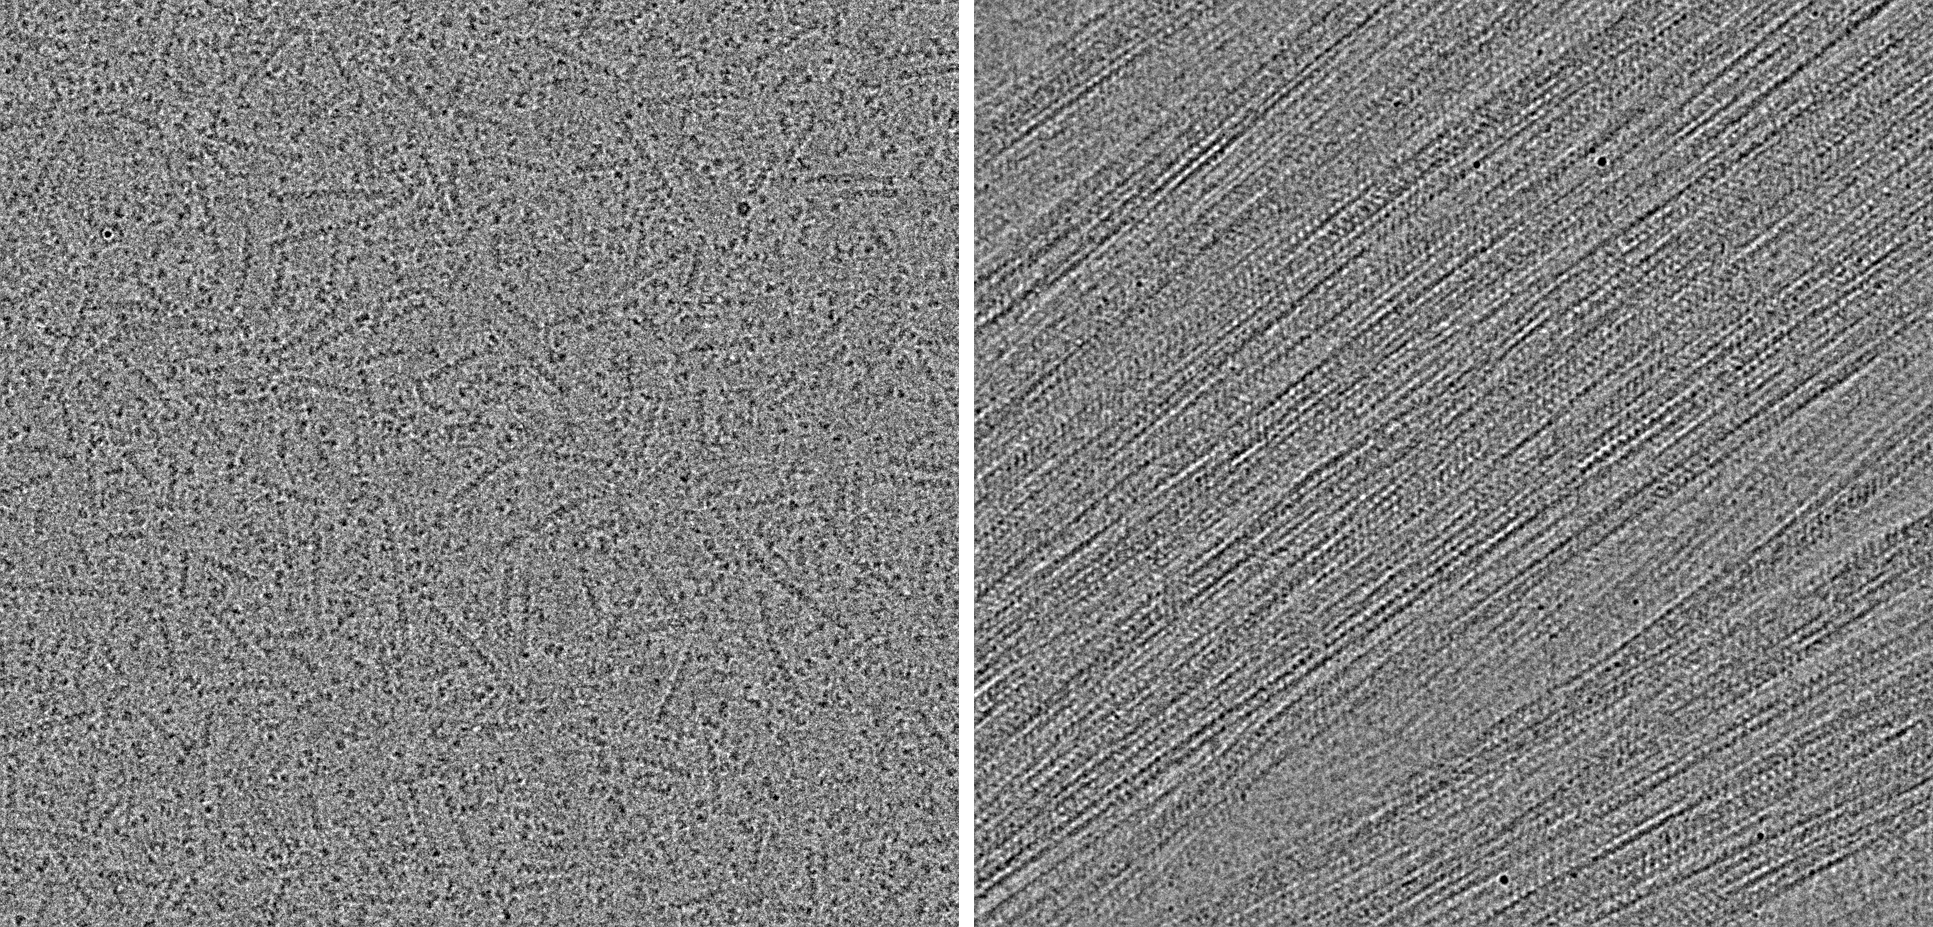
\includegraphics[width=\textwidth]{other/ftsz_mics.png}
    \titledcaption[Micrographs of FtsZ filaments]{Micrographs containing FtsZ filaments. When filaments are individual and well separated (left) they are ideal for picking and refinement. In some cases, FtsZ filaments form bundles (right) which are harder to pick, refine and classify due to the overlapping particles.}
    \label{fig:ftsz_micrographs}
\end{figure}

% TODO: data collection...?
We used CryoSPARC~\cite{punjaniCryoSPARCAlgorithmsRapid2017} for filament picking, which gave us a large amount of particles (>4M) to classify and clean up from spurious picks.
After cleaning, we ended up with about 2M particles, and very uniform classes with little variation (\autoref{fig:ftsz_classes}).
This is a typical symptom of strong preferential orientation due to the air-water interface (\fullref{em_pref_ori}), leading to a very limited range of views in the particle projections.
Although we saw hints of different views in the bundled filaments, they proved impossible to disentangle enough to obtain well-resolved classes.

\begin{figure}[ht]
    \centering
    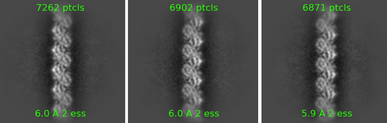
\includegraphics[width=\textwidth]{other/ftsz_classes_untilted.png}
    \titledcaption[FtsZ filament: 2D classes]{Classification results from particles with strong preferential orientation. All classes show very similar views of the FtsZ filaments, with minor variation in the out-of-plane angle.}
    \label{fig:ftsz_classes}
\end{figure}

Given the strong preferential orientation, it's unsurprising that 3D reconstructions from these particles showed very strong resolution anisotropy (while reporting \sim4 Å global resolution), so much so that we couldn't convincingly fit the monomeric model in the map (\autoref{fig:ftsz_map_bad}).

\begin{figure}[ht]
    \centering
    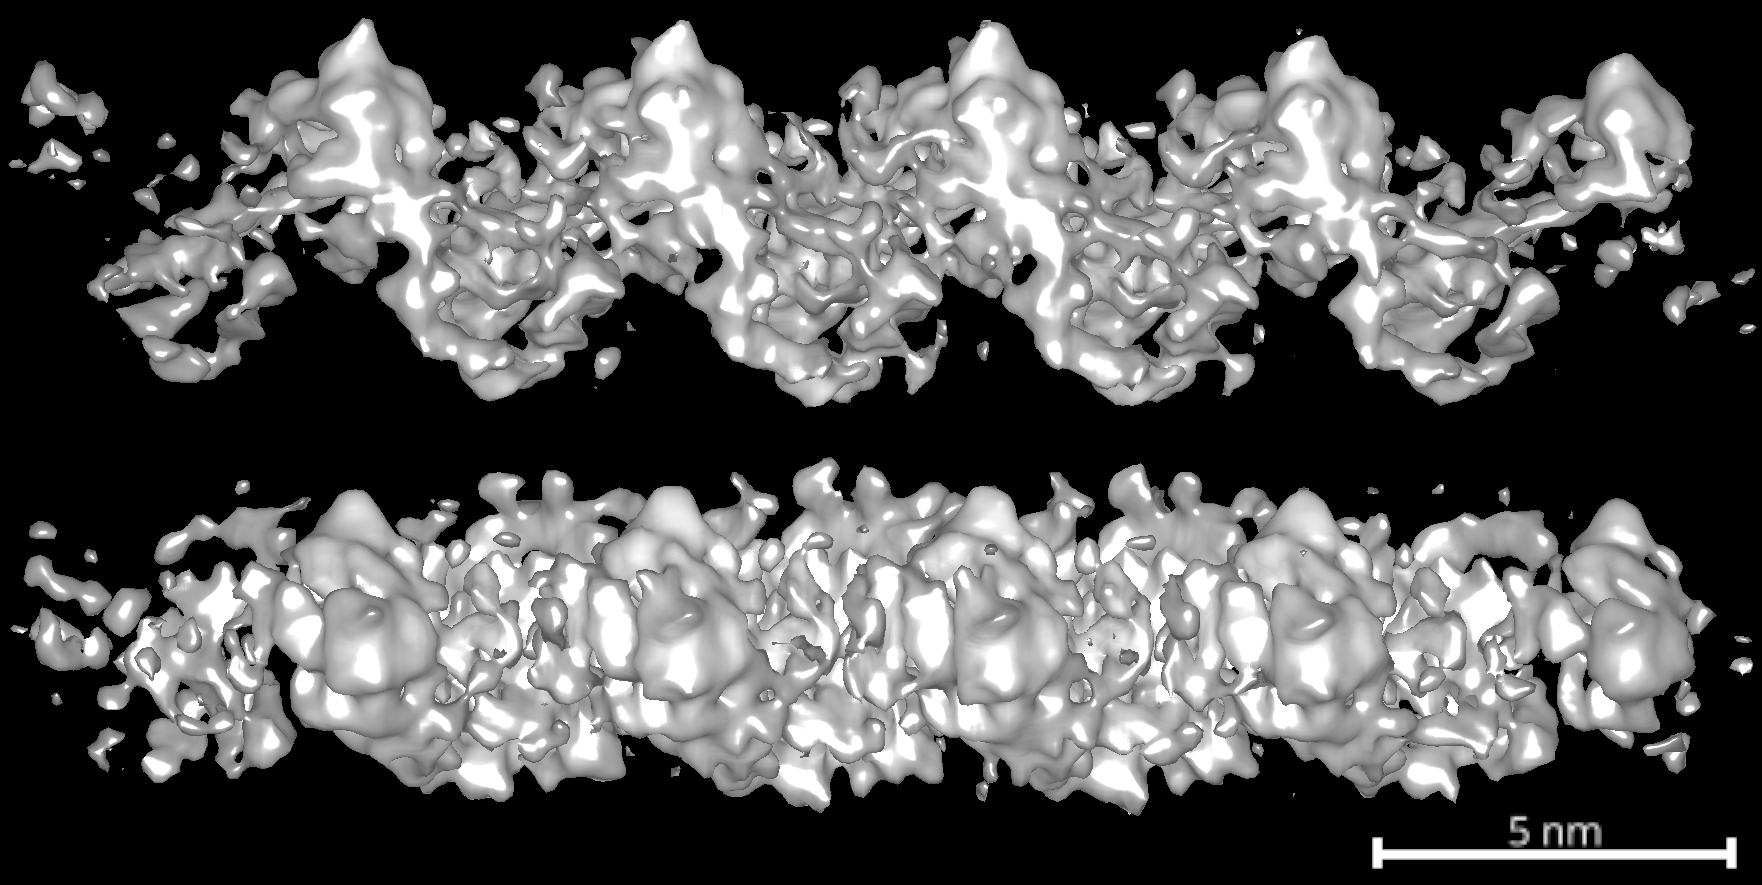
\includegraphics[width=\textwidth]{other/ftsz_map_bad.png}
    \titledcaption[FtsZ filament: anisotropic map]{FtsZ filament map affected by preferential orientation, viewed from the same direction as most 2D classes (top) and rotated by 90° (bottom) to highlight the streaking artifacts due to anisotropic orientation sampling.}
    \label{fig:ftsz_map_bad}
    % TODO: add pref orientation proof (orientation map or so)
\end{figure}

The best map currently available of FtsZ filaments (from \textit{Klebsiella pneumoniae}) also suffered from similar issues, despite the high reported resolution (\sim3 Å)~\cite{fujitaStructuresFtsZSingle2023}.

We attempted to address the issue of preferential orientation in two different ways: collecting a tilted dataset of the same samples, and preparing a new sample with methods that combat air-water interface effects.

\subsubsection{Graphene and streptavidin-coated grids}

We attempted to address the preferential orientation problem by using functionalized graphene grids~\cite{luFunctionalizedGrapheneGrids2022}, and streptavidin-coated affinity support grids~\cite{crucifixImmobilizationBiotinylatedDNA2004,hanLongShelflifeStreptavidin2016}.
While these approaches have been shown to work, we struggled to obtain usable grids; in the meantime, the sample prepared with the addition of detergent showed promising results, so we moved forward with it instead.

\subsubsection{Tilted data collection}\label{ftsz_tilted}

We prepared the sample in the same way, but this time the data collection was done with the grid at a 35° tilt.
Following the same workflow as with the untilted dataset, we then picked, classified and selected particles, obtaining a new set of class averages (\autoref{fig:ftsz_classes_tilted}).
These classes where immediately more promising than the ones from the untilted datasets, showing multiple views from the first round of classification, even in isolated filaments. % TODO: explain why these classes where better, did we get more, explain figure, what we were looking for, etc

\begin{figure}[ht]
    \centering
    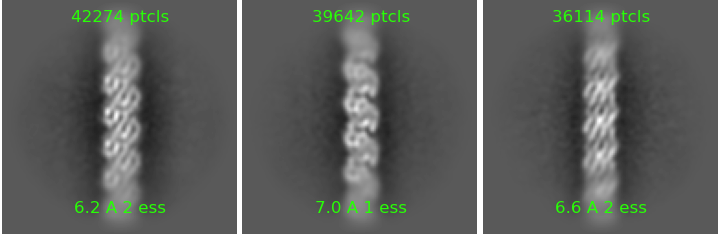
\includegraphics[width=\textwidth]{other/ftsz_classes_tilted.png}
    \titledcaption[FtsZ tilted dataset: 2D classes]{Classification results from the tilted dataset. Differently from the untilted classes, particles successfully classified into distinct views of the filament.}
    \label{fig:ftsz_classes_tilted}
\end{figure}

Despite the better view distribution of 2D classes, our 3D reconstructions had the same anisotropy issues as the untilted data.
Assuming a unform distribution of in-plane angles of the filaments (which we observed in the original dataset), a single, relatively high-tilt dataset should cover a higher portion of 3D fourier space during backprojection and thus significantly improve map isotropy~\cite{tanAddressingPreferredSpecimen2017}.

With preferentially oriented filaments collected at a fixed tilt angle, there should be a strong correlation between in-plane angle (easily identifiable from the micrograph) and the projection view (which is identified by classification). % TODO: show with synthetic dataset? Also, could it be that multiple euler combinations are redundant and correlation was just bad? How did I do this thing again?
Upon closer inspection of the picking data, however, we observed that the out-of-plane angles assigned to each particle showed no correlation with the assigned 2D class (\autoref{fig:ftsz_class_angles}).

\begin{figure}[ht]
    \centering
    \includegraphics[width=\textwidth]{example-image.png}
    \titledcaption[Out-of-plane angle by class in FtsZ titled dataset]{Out-of-plane angle plotted against the assigned 2D class. TODO}
    \label{fig:ftsz_class_angles}
\end{figure}

We soon realized that the 3D reconstruction routines of both Relion~\cite{scheresRELIONImplementationBayesian2012} and CryoSPARC~\cite{punjaniCryoSPARCAlgorithmsRapid2017} were struggling with assigning Euler angles, resulting in practically random orientations.
To impose more constraints on the refinement based on this prior knowledge on the geometry of the system, we calculated the theoretical orientation of each particle based on the in-plane angle (and assuming perfect preferential orientation), which we then used to initialize the particle poses (\fullref{stemia_angles}).

Unfortunately, this approach did not yet bear fruits: CryoSPARC does not provide fine control over angle priors and search patterns, and Relion's parameters for angle refinement proved tricky to control and resulted in orientations being either stuck in local minima, or fully randomized again (\autoref{fig:ftsz_angle_dist}).

\begin{figure}[ht]
    \centering
    \includegraphics[width=\textwidth]{example-image.png}
    \titledcaption[Angle distribution after 3D reconstruction in FtsZ tilted dataset]{TODO: angle distribution plot}
    \label{fig:ftsz_angle_dist}
\end{figure}

\subsubsection{Addition of detergent}
Detergent has long been used as a way to address preferential orientation and aggregation of proteins in the sample.
In our case, while it did not affect the orientation problem, it allowed FtsZ to polymerize into longer filaments without creating large bundles (\autoref{fig:ftsz_ddm_mics}).

\begin{figure}[ht]
    \centering
    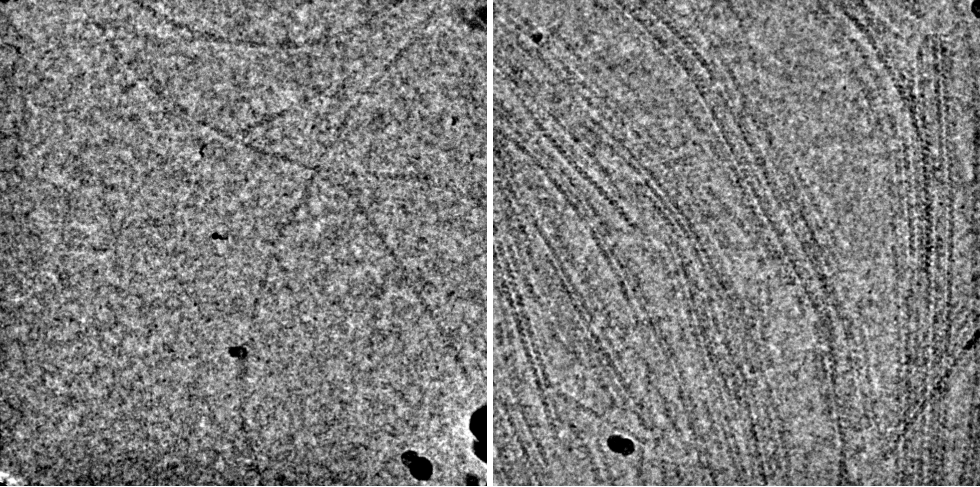
\includegraphics[width=\textwidth]{other/ftsz_mics_ddm.png}
    \titledcaption[Micrographs of FtsZ with detergent]{The addition of detergent allowed the FtsZ filaments to elongate further, without resulting in dense bundles (left). When bundles formed (right), they were often less densely packed than without detergent, opening up the possibility to pick bundled filaments in order to investigate side interactions.}
    \label{fig:ftsz_ddm_mics}
\end{figure}

The longer filaments and the very small helical twist (estimated at <1° with the previous samples), should result in different side views of the monomers being visible in the dataset.
Indeed, we observe a higher diversity in classification results, including classes with different views of single filaments (\autoref{fig:ftsz_ddm_classes_single}) and classes with two or three filaments interacting side-by-side (\autoref{fig:ftsz_ddm_classes_double}).

\begin{figure}[ht]
    \centering
    \begin{subfigure}[B]{.5\textwidth}
        \centering
        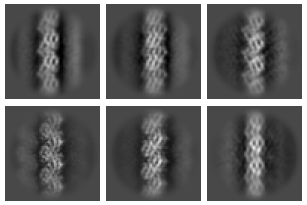
\includegraphics[width=\textwidth]{other/ftsz_classes_single.png}
        \caption{Classes with different views on single FtsZ filaments.}
        \label{fig:ftsz_ddm_classes_single}
    \end{subfigure}%
    \hfill
    \begin{subfigure}[B]{.5\textwidth}
        \centering
        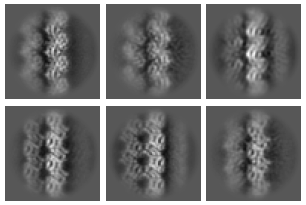
\includegraphics[width=\textwidth]{other/ftsz_classes_double.png}
        \caption{Classes with multiple interacting FtsZ filaments.}
        \label{fig:ftsz_ddm_classes_double}
    \end{subfigure}%
    \titledcaption[2D classes of FtsZ with detergent]{TODO: ftsz ddm classes}
    \label{fig:ftsz_ddm_classes}
\end{figure}

This project has now been taken over by Harald Bernhard, a postdoc in the MICA group, who already managed to further improve the map in a few ways.
With careful use of 2D and 3D classifications, it's possible to better isolate single filaments, which improves the initial model generation.
Balancing the different views by number of particles also improves the orientation distribution, reducing map artifacts at the cost of some global resolution.
Additionally, the use of a bigger box size in particle extraction has improved slightly the quality of the alignements and 2D class averages.
While the anisotropy issue remains, the new maps are much more interpretable, and match those by \citet{fujitaStructuresFtsZSingle2023} from \textit{K. pneumoniae} FtsZ (\autoref{fig:ftsz_hari_map}).

\begin{figure}[ht]
    \centering
    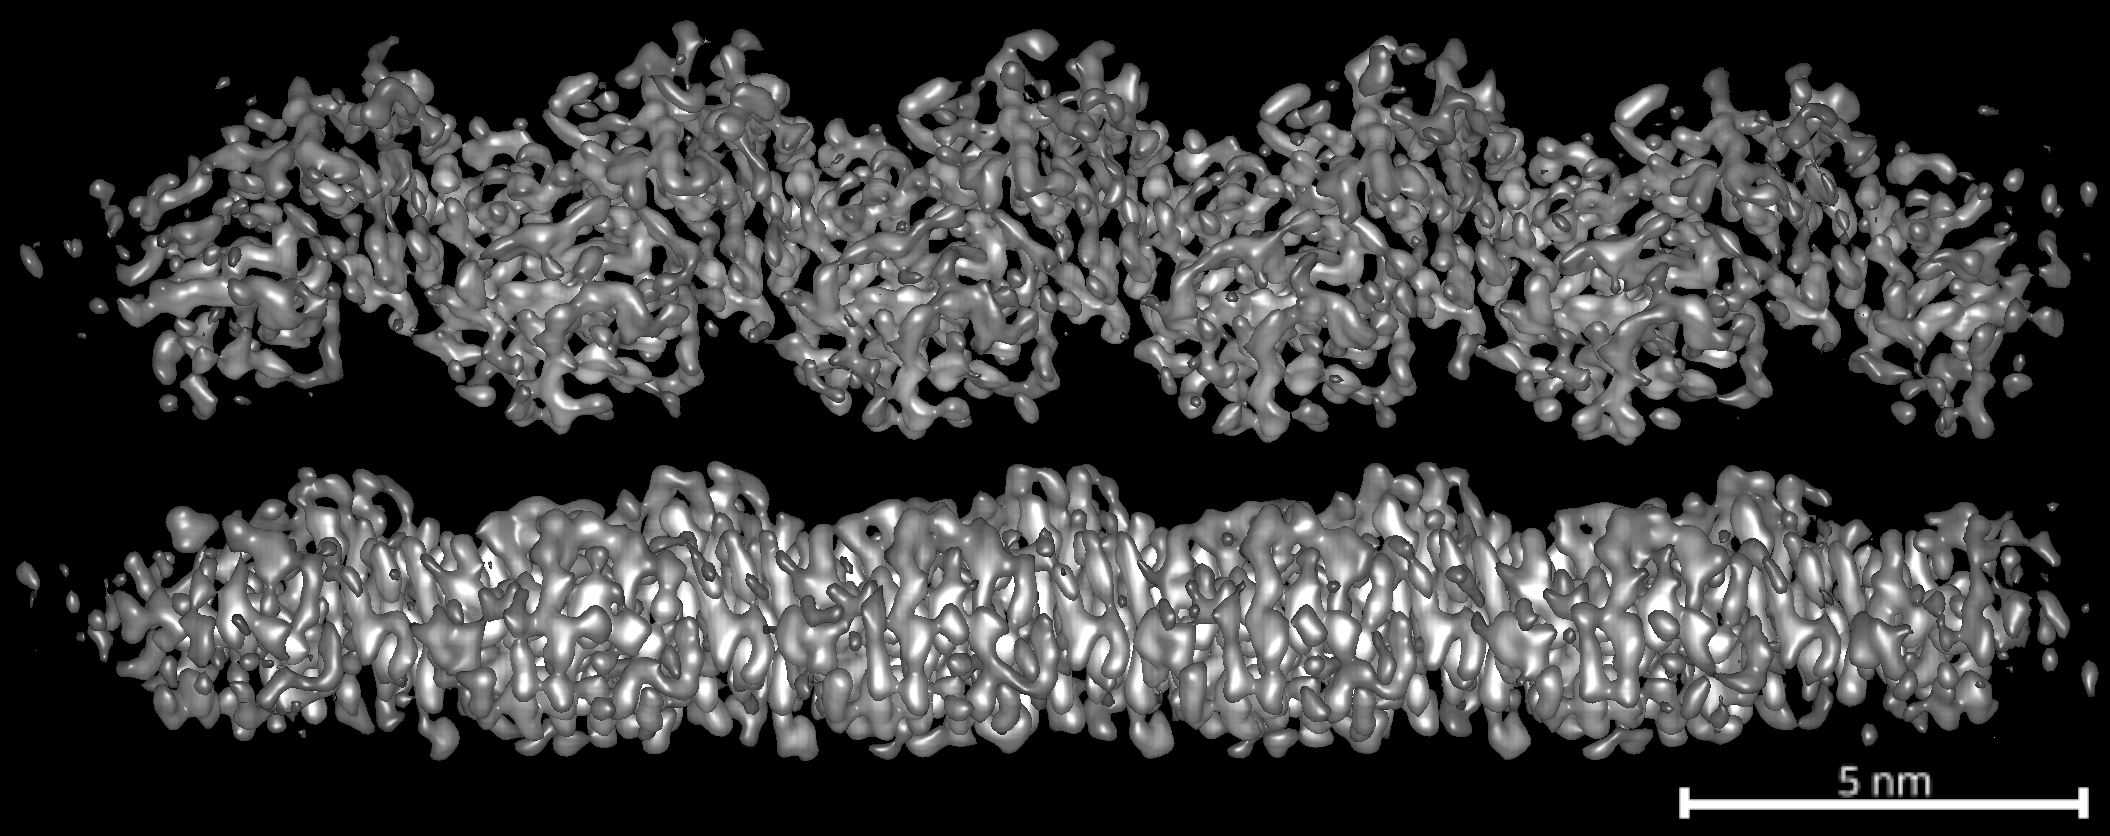
\includegraphics[width=\textwidth]{other/ftsz_map_good.png}
    \titledcaption[3D map of FtsZ with detergent]{Using the FtsZ+DDM dataset, and more careful 2D and 3D classifications to clean the dataset and better balance different views, Harald significantly improved on the FtsZ filament map. Preferential orientation is unfortunately still not fully solved, as evidenced by the streaking artifacts along one direction (bottom view), which are not present in the other (top view).}
    \label{fig:ftsz_hari_map}
\end{figure}

\subsection{Tomography and STA}

In parallel to the study of \textit{in vitro} FtsZ filament by SPA, we also investigated the FtsZ \textit{in situ} in the tomograms of \textit{D. radiodurans} lamellae.
Some of our findings and speculations about the 3D morphology of FtsZ are included in the \textit{D. radiodurans} manuscript (\fullref{drad_ftsz} and \fullref{ftsz_discussion}).

Our observations on the reconstructed tomograms matched those by \citet{sextonSuperresolutionConfocalCryoCLEM2022}, who also used tomography to look into D.rad and identified FtsZ and FtsA forming filaments just below the inner membrane of the septal tips (\autoref{fig:ftsz_tomo_slice}). % TODO: show more examples of this, how many have it, etc...

\begin{figure}[ht]
    \centering
    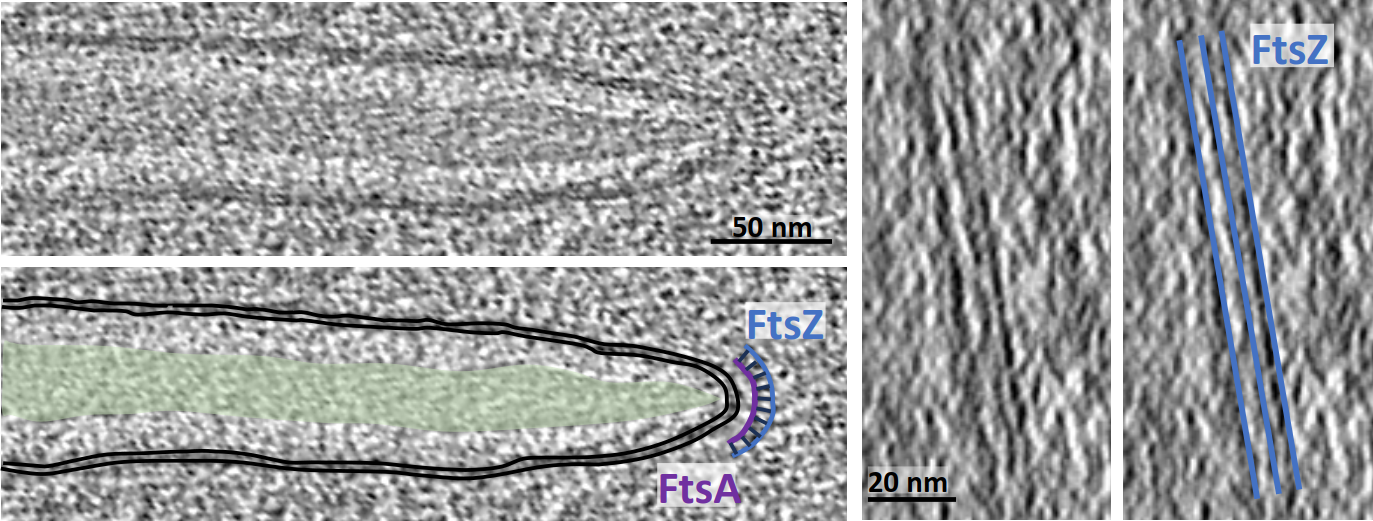
\includegraphics[width=\textwidth]{other/ftsz_slices.png}
    \titledcaption[FtsZ: tomogram slices from top and side view]{When viewing a cross-section of the bundle at the tip of the septa of \textit{D. radiodurans} (left), FtsZ is visible as a double arch separated by a gridded pattern. This is likely the result of a layer of FtsA bridging between the membrane and a layer of FtsZ filaments. (figure adapted from \autoref{drad_fig4}).}
    \label{fig:ftsz_tomo_slice}
\end{figure}

The size and spacing between FtsZ filaments is generally consistent with crystal structures and SPA studies on FtsZ filaments~\cite{mcquillenInsightsStructureFunction2020}.
the distance between FtsZ+FtsA filaments and the membrane in our tomograms is consistent with the expected \sim13-16~\cite{mcquillenInsightsStructureFunction2020}.
However, the width of the bundle appears to be smaller than the previously found 80-100 nm~\cite{mcquillenInsightsStructureFunction2020}, typically no wider than around 50-60 nm; this might be caused by differences in the thickess of the septa or modes of septation between different bacteria.

\subsubsection{Subtomogram averaging}

While it is clear that FtsZ and FtsA are forming filaments and bundles in vitro, and that they localize to the Z-ring in a bundle-like fashion, the details of this superstructural assembly are unknown.
To get a higher resolution view of this complex \textit{in situ}, we performed STA on particles picked from the FtsZ arches at the tips of the septa (\autoref{fig:ftsz_tomo_slice}).

Given the apparent regularity of the bundles (whose morphology appears unchanged across their length), we used blik's surface picking tool~\cite{gaifasBlikExtensible3D2024,gaifasBlikPythonTool2024}, which allows us to distribute regularly spaced particles on the sheet-like FtsZ bundles.
The inter-particle distance was chosen based on the smallest distance in the regular comb-like dark/light pattern along the FtsZ arches. % TODO: how many particles?
Two different sets of particles were thus generated: with inter-particle distance matching the visible pattern (\sim50 Å), and twice oversampled (\sim25 Å) (\autoref{fig:ftsz_tomo_picks}).

\begin{figure}[ht]
    \centering
    \begin{subfigure}[B]{.49\textwidth}
        \centering
        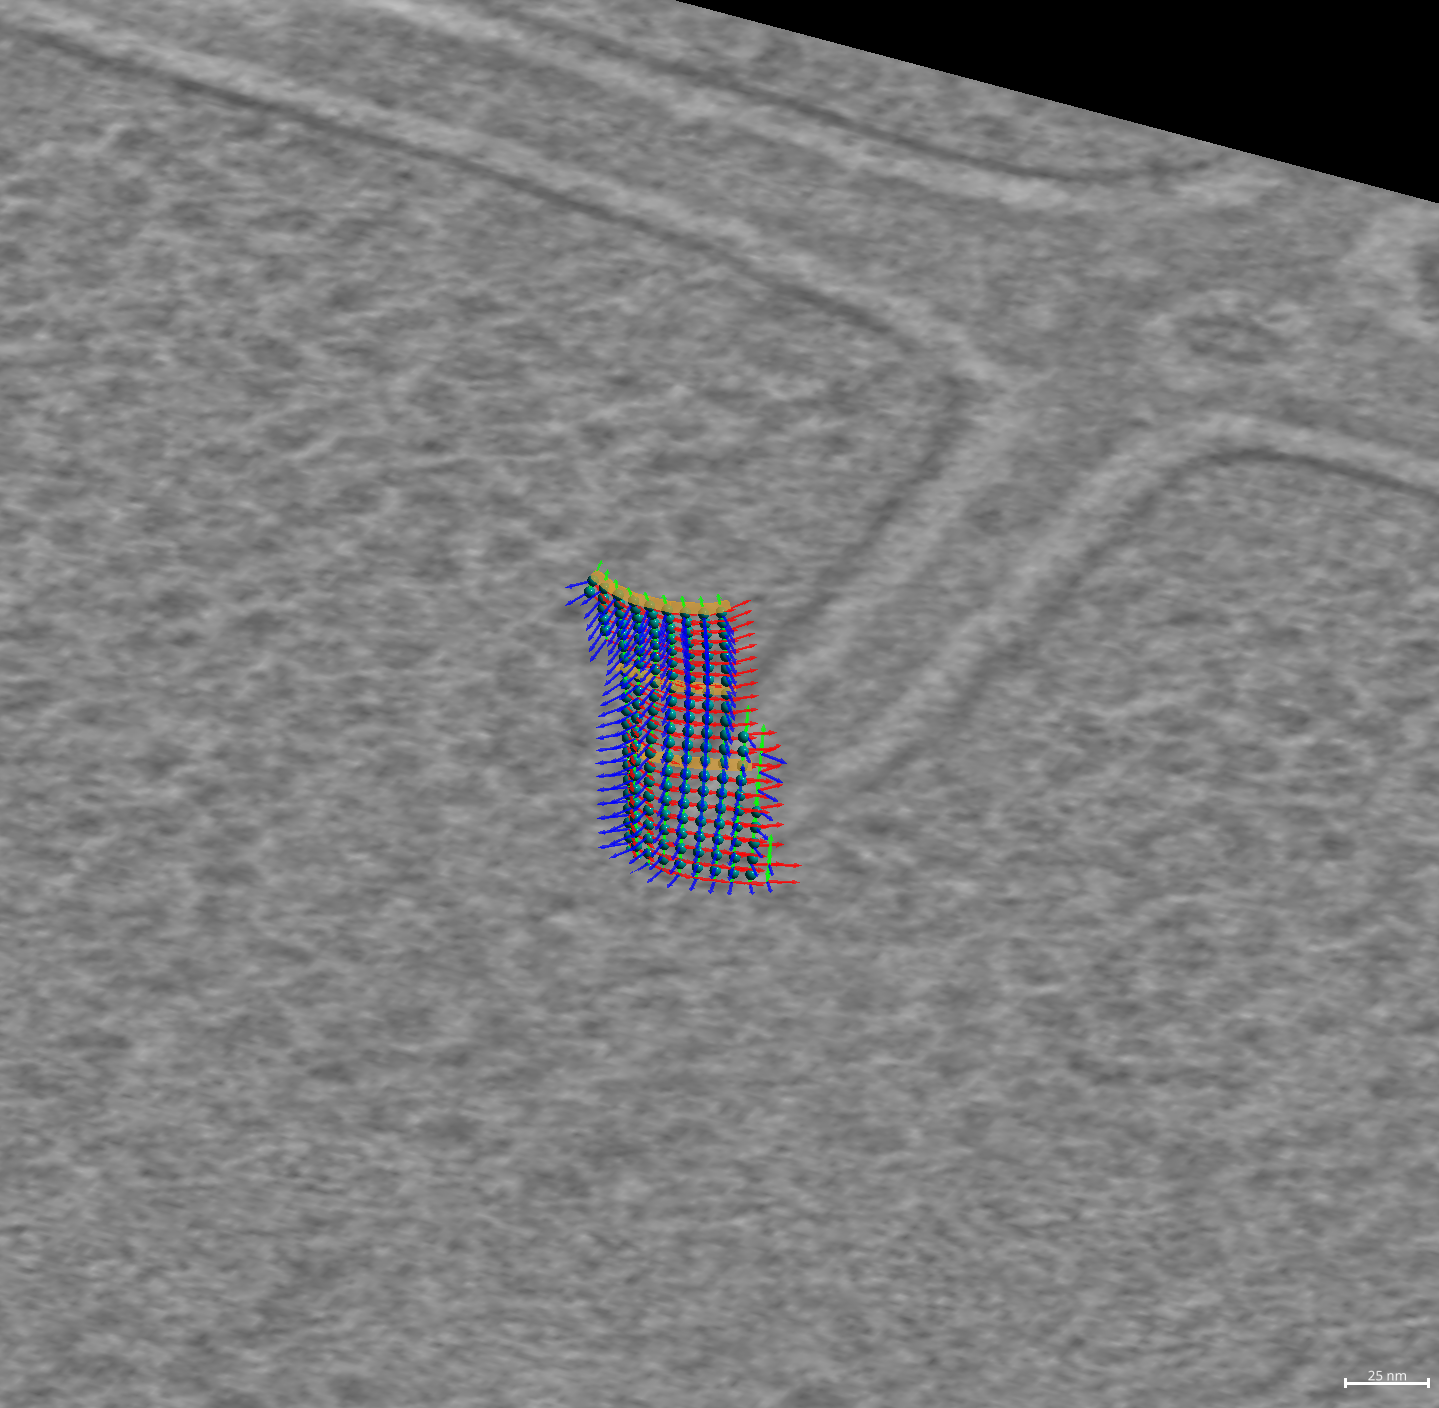
\includegraphics[width=\textwidth]{other/ftsz_particles_50A.png}
        \caption{Particle picks at 50 Å spacing.}
        \label{fig:ftsz_tomo_picks_50}
    \end{subfigure}%
    \hfill
    \begin{subfigure}[B]{.49\textwidth}
        \centering
        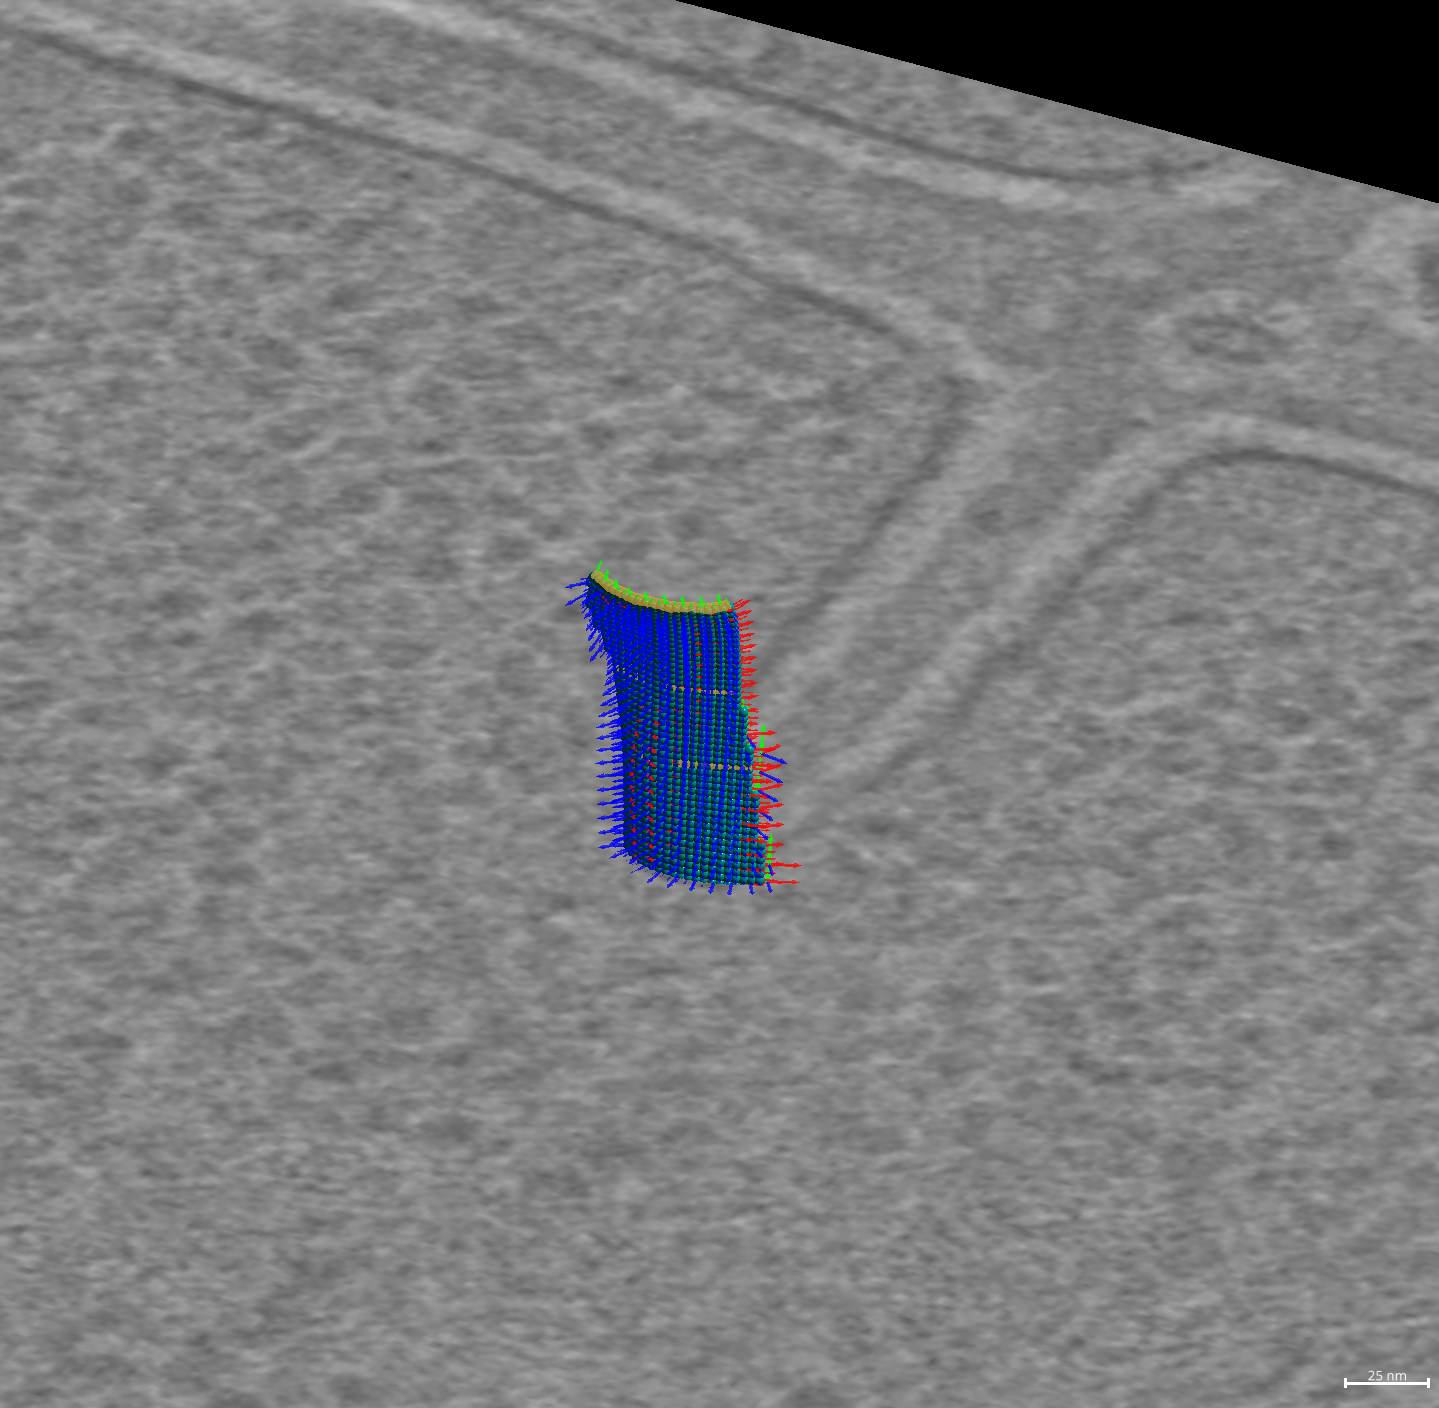
\includegraphics[width=\textwidth]{other/ftsz_particles_25A.png}
        \caption{Particle picks at 25 Å spacing.}
        \label{fig:ftsz_tomo_picks_25}
    \end{subfigure}%
    \titledcaption[Surface-based FtsZ particle picks for STA]{Particle picks on FtsZ at the tip of the septa in \textit{D. radiodurans} tomograms, generated with surface-based picking in blik~\cite{gaifasNaparipropertiesplotter2021,gaifasBlikPythonTool2024} at two different inter-particle spacings.}
    \label{fig:ftsz_tomo_picks}
\end{figure}

Subtomograms were reconstructed in Warp~\cite{tegunovRealtimeCryoelectronMicroscopy2019} using these particle picks, at different resolutions and with varying box sizes.
Using Relion~\cite{scheresRELIONImplementationBayesian2012,zivanovBayesianApproachSingleparticle2022,burtImageProcessingPipeline2024}, we performed subtomogram averaging and 3D classification to refine the positions and obtain a 3D map of the particles.
Due to the low magnification of the dataset (Nyquist \simeq9 Å), Relion was in most cases struggling to assign orientations.
The only refinement that resulted in consistent orientations and a reasonable map was with particles picked at 50 Å spacing, and subtomograms reconstructed at the highest resolution (4.346 Å/px) and with a large box size of 64 pixels, corresponding to \sim28 nm (\autoref{fig:ftsz_subtomo}).

\begin{figure}[ht]
    \centering
    \begin{subfigure}[B]{.49\textwidth}
        \centering
        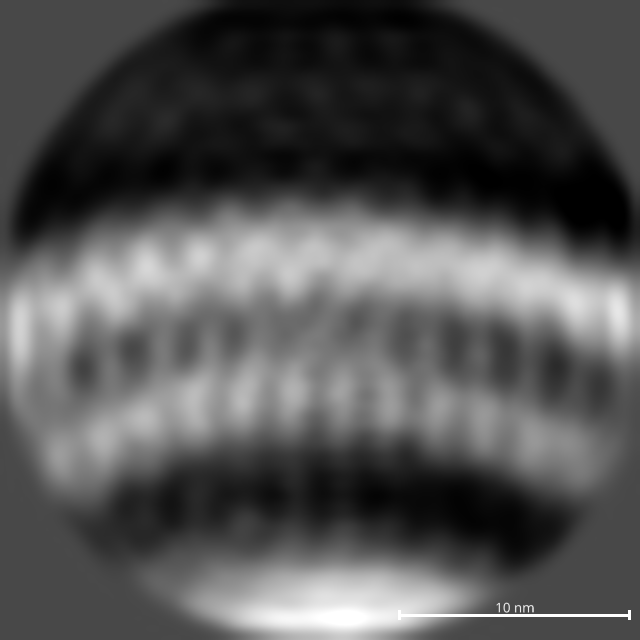
\includegraphics[width=\textwidth]{other/ftsz_subtomo_slice.png}
        \caption{Z-slice through the best FtsZ subtomogram.}
        \label{fig:ftsz_subtomo_slice}
    \end{subfigure}%
    \hfill
    \begin{subfigure}[B]{.49\textwidth}
        \centering
        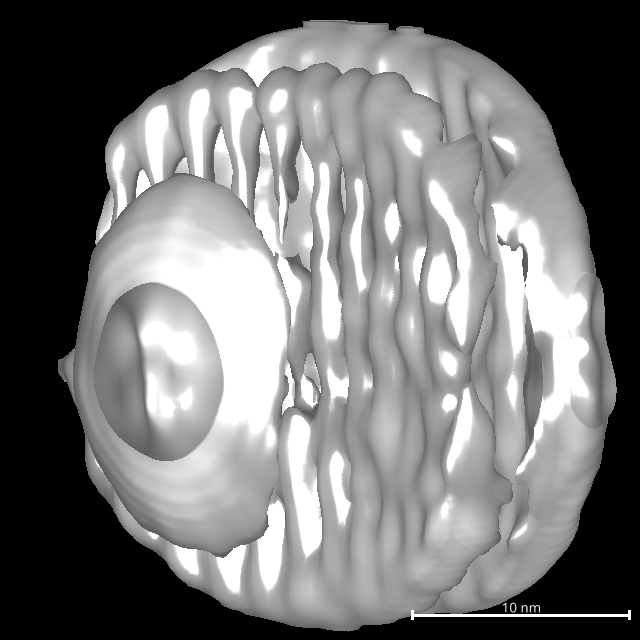
\includegraphics[width=\textwidth]{other/ftsz_subtomo_iso.png}
        \caption{Isosurface of the best FtsZ subtomogram.}
        \label{fig:ftsz_subtomo_iso}
    \end{subfigure}%
    \titledcaption[FtsZ STA preliminary results]{Subtomogram averaging results of the particle picks on FtsZ at the tip of the septa in \textit{D. radiodurans}. The grid-like pattern visible in the tomogram slices is captured by the subtomograms, but the resolution is too low for further interpretation.}
    \label{fig:ftsz_subtomo}
\end{figure}

It's worth noting that due to the nature of the division cycle of \textit{D. radiodurans}, the bacterium is generally found as a tetrad laying flat on the grid, which leads to a preferential orientation of the septa (and therefore the FtsZ filaments) along the Z axis on the tomograms.
Due to the missing wedge (\fullref{et_tomo_reconstruction}), along which the filaments are aligned, the information is blurred along the FtsZ filament axis, limiting for example the ability to distinguish individual FtsZ monomers.

\subsection{Materials and Methods}\label{ftsz_methods}

\subsubsection{Sample preparation for SPA}

\paragraph{FtsZ only}
5μl FtsZ at 12.5 mg/ml were diluted in 4 μl buffer (50 mM Tris-HCl pH 8.0, 200 mM NaCl), and 1 μl GpCpp at 10 mM.
Mix was then incubated at 25°C for 75 min to allow for filament elongation.
4μl of mix was then diluted in 16 μl of buffer (50 mM Tris-HCl pH 8.0, 200 mM NaCl), and 1 μl GpCpp at 10 mM.
The sample was then immediately frozen on R2/1 300mesh EM grids (blot time: 3.5 s).

\paragraph{FtsZ+DDM}
2μl FtsZ at 12.5 mg/ml were diluted in 16 μl buffer (50 mM Tris-HCl pH 8.0, 200 mM NaCl), and 2 μl GpCpp at 10 mM.
Mix was then incubated at 25°C for 30 min to allow for filament elongation, after which 2μl DDM at 0.09\% was added.
Grids were frozen with and without further 5x dilution in buffer (50 mM Tris-HCl pH 8.0, 200 mM NaCl, 1 mM GpCpp, 0.009\% DDM: 2 μl mix + 8 μl buffer)

TODO: should we include details about reproducibility/elongation? I added some to the text above, but maybe we need more details here.

TODO: graphene and streptavidin grids

\subsubsection{Data Collection for SPA}

TODO: I need help here for the technical microscopy details...

\subsubsection{SPA processing}

TODO: filament picking (parameters, issues with length)

link to \fullref{stemia_angles}.

\subsubsection{\textit{D. radiodurans} lamellae and tomography data collection}

See \fullref{drad_lamellae_method} and \fullref{drad_tomo_method}.

\subsubsection{STA data processing}

TODO: blik, relion


\section{Tools and scripts}

\subsection{waretomo}\label{waretomo}

As most cryo-ET users, over time I kept tweaking and improving my processing pipeline.
At present, it consists of three main elements: Warp~\cite{tegunovRealtimeCryoelectronMicroscopy2019} for preprocessing and tomogram and subtomogram reconstruction, AreTomo~\cite{zhengAreTomoIntegratedSoftware2022} for tilt series alignment, and Relion~\cite{scheresRELIONImplementationBayesian2012,zivanovBayesianApproachSingleparticle2022,burtImageProcessingPipeline2024} for STA.

To facilitate batch processing and remove most needs for manual intervention (and potential points of failure), I developed an automated tool which connects Warp to AreTomo: \href{https://gihub.com/brisvag/waretomo}{waretomo}~\cite{gaifasWaretomo2024}.

Specifically, waretomo:
\begin{enumerate}[noitemsep]
    \item automates parsing \texttt{.mdoc} files to provide appropriate inputs to AreTomo
    \item ensures that tilts skipped in Warp are properly handled
    \item adjusts tilt angles in Warp based the otuput of AreTomo to untilt tilted samples (such as lamellae)
    \item optionally reconstructs preliminary tomograms with AreTomo and denoises them with Topaz~\cite{beplerTopazDenoiseGeneralDeep2020}
\end{enumerate}

When possible, each step is performed in parallel (and on GPUs) to maximize resource usage and minimize idle time.
While this tool is available and open source, it's not yet publication-ready and still in alpha, so bugs are expected.

\subsection{emscan}

In cell-extract cryo-EM~\cite{suBuildRetrieveMethodology2021,kyrilisIntegrativeBiologyNative2019}, a dataset may contain a large variety of proteins and complexes, many of which unknown.
In these non-purified datasets, automating parts of the selection and protein identification processes is essential for practical applications such as structural proteomics of a novel organism.

As a contribution to the PhD project of Eymeline Pageot --- another PhD student in the MICA group under the supervision of Ambroise Desfosses --- I developed \href{https://gihub.com/brisvag/emscan}{emscan}, a napari~\cite{thenaparicommunityNapariMultidimensionalImage2024}-based tool that searches the EMDB database~\cite{thewwpdbconsortiumEMDBElectronMicroscopy2024} for maps whose projections have a high similarity with the input 2D classes.

This allows for example to discard classes from already-solved structures, or to identify 2D classes that potentially belong to different views of a protein whose homologues are present on the EMDB.

% TODO explain how it works

% \1 projection matching for eymeline's work
%     \2 more native than SPA but more straightforward than STA
%     \2 would be cool to go into some technical details here (cross-correlation, projection, etc)
%     \2 optimizing for space and performance
%     \2 the issues around cross correlation

\subsection{Other napari tools}

During my thesis, napari proved time and time again a powerful library for creating custom interactive visualisation tools.
Some smaller napari-based tools and plugins I contributed to that are worthy of mention are:

\begin{enumerate}
    \item \href{https://github.com/cellcanvas/surforama}{surforama}~\cite{yamauchiSurforamaInteractiveExploration2024}, a tool to explore cryo-ET membrane annotations inspired by membranorama~\cite{tegunovDtegunovMembranorama2024}, fruit of a collaboration with other napari developers and members of the teamtomo community
    \item \href{https://github.com/brisvag/napari-molecule-reader}{napari-molecule-viewer}, a plugin to open PDB and mmCIF files in napari
    \item a \href{https://github.com/napari/napari/blob/main/examples/fourier_transform_playground.py}{fourier transform playground} to interactively explore the relationship between images and their FTs
    \item a \href{https://gist.github.com/brisvag/d6394d05b2f994e083ec279d6976484f}{Euler angle playground} to build an intuition on the various Euler angle conventions and their effects on particle orientations
\end{enumerate}

\subsection{cs2star}

A small tool, but used widely by our group and others, and later \href{https://sbgrid.org/software/titles/cs2star}{added to SBGrid}~\cite{morinCuttingEdgeCollaboration2013}, \href{https://github.com/brisvag/cs2star}{cs2star}~\cite{gaifasCs2starPy2021} is a small wrapper around the widespread \href{https://github.com/asarnow/pyem}{cryosparc2star.py} which automates a few tedious manual steps normally needed when converting CryoSPARC~\cite{punjaniCryoSPARCAlgorithmsRapid2017} projects to Relion~\cite{scheresRELIONImplementationBayesian2012} ones.

\subsection{stemia}

\href{Stemia}{https://github.com/brisvag/stemia} is a collection of command-line tools that I developed but that were either too small or too niche to make sense as standalone packages.

\subsubsection{Out-of-plane angle generation}\label{stemia_angles}
This tool was developed to work on the FtsZ tilted dataset (\fullref{ftsz_tilted}). % TODO: expand
